\section{Ejercicio 4}

\subsection{Enunciado}
El enunciado nos pide, dada una arreglo de tamaño N de matrices de 3x3 , un a matriz de 3x3 M y un numero L, decidir
si existe un subarreglo de largo L que al multiplicarlo nos de M.
Ademas todas las matrices del problema tienen sus elementos en Z100007

\subsection{Formalizando}
Reformulando, dado un arreglo a1...an de con elementos en Z3x3 100007, queremos ver si existen indices
i, j tal que j - i == L y ai x ai+1 x .... x a j-1 == M

\subsection{Algunas propiededades}
Lo primero que debemos recordar para resolver este problema es que, la multiplicacion de matrices es asociativa.
Como en muchos problemas en la computación, vamos a querer resolver ''subproblemas''
que nos ayuden a resolver el problema original. Así, nos será útil saber que si encontramos dos subarreglos tales que:
ai x ai+1 ... x ak = T1 y ak+1 x ... x aj = T2 y T1 * T2 = M, donde i y j
respetan lo mencionado en el punto anterior..
encontramos lo que buscabamos.
\newline
Para ser más breves, denotemos como subarreglo \textbf{ganador} a un subarreglo que cumple las condiciones que buscamos.
Con la idea en mente de buscar subproblemas para resolver el problema original, dividamos el arreglo en dos.
Notamos que si al arreglo original lo dividimos, entonces se pueden dar los siguientes casos:
\begin{itemize}
\item Hay un subarreglo ganador totalmente contenido en la primer mitad.
\item Hay un subarreglo ganador totalmente contenido en la segunda mitad.
\item Hay un subarreglo ganador que esta parcialmente contenido en cada una de las mitades.
\item No hay subarreglo ganador, asi que la respuesta seria ''NO''.
\end{itemize}

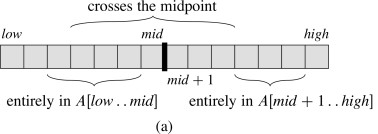
\includegraphics{img/subarrays-casos.jpg}

Facilmente podemos ver que si resolvemos el tercer caso, es decir, cuando un subarreglo
ganador esta parcialmente contenido en cada mitad, podriamos dar un algoritmo
que utilice la técnica de ''Divide And Conquer'' para resolver el problema.

\subsection{Prefijos y sufijos}
Si dividimos un arreglo en dos mitades, y queremos buscar si existe un subarreglo ganador
parcialmente contenido en cada mitad, entonces tendremos que buscar si algun subarreglo
sufijo de la primer mitad, al concatenarse con un subarreglo prefijo de la segunda mitad,
resulta ganador.
Para el algoritmo que vamos a realizar, hay que tener en cuenta que si utilizamos un
sufijo de tamaño i, solo debemos probar con un prefijo de tamaño L - i, pues es el unico prefijo
que nos puede dar el tamaño L en la concatenación.

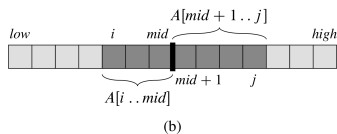
\includegraphics{img/subarrays-crossmid.jpg}

En una pasada lineal, podemos precomputar todos los prefijos (el resultado de su multiplicacion),
y los guardamos en un arreglo prefijo[i], que almacena el resultado del prefijo de tamaño i.
\newline
En otra pasada lineal, vamos computando el resultado de multiplicar todo un sufijo, aumentando
el tamaño del sufijo cada iteracion. Asi, si tenemos el sufijo de tamaño i, chequeamos si
la multiplicacion con el prefijo de tamaño L - i nos da M, es decir:
\newline
$sufijo * prefijo[L - i] = M$
\newline
Chequeando con todos los sufijos de tamaño menor a L, resolvemos la etapa de ''Conquista'' de nuestro
algoritmo.

\subsection{Pseudocódigo}

\begin{algorithmic}


\Function{haySubarreglo}{i, j, matrices, M, L}
  \If {$j - i < L$}
    \State \Return{false}
  \EndIf

  \If{$j - i == 1$}
    \State \Return {matrices[i] == M}
  \EndIf
    
  \State 
  
  \State res $\gets$ false
  \State mid $\gets$ (start + end) / 2
  \State prefix[l+1] $\gets$ \{...\}
  \State prefix[0] $\gets$ $I$\textsubscript{3x3}
  
  \State 
  
  \State i $\gets$ 0
  \While{i $\leq$ l \textbf{and} mid + i - 1 $\textless$ end}
    \State prefix[i] $\gets$ prefix[i - 1] * matrices[mid + i - 1];
    \State i++
  \EndWhile
  
  \State
  \State suffix $\gets$ $I$\textsubscript{3x3}
  \State
  
  \State i $\gets$ 1
  \While {$i$ $\leq$ l \textbf{and} mid - i $\geq$ start}
    \State suffix $\gets$ suffix * matrices[mid - i]
    \If {suffix * prefix[l - i] = m}
      \State res $\gets$ true
    \EndIf
    \State i++
  \EndWhile
  
  \State
  
  \State res $\gets$ res \textbf{or} haySubsecuencia(start, mid, matrices, m, l)
  \State res $\gets$ res \textbf{or} haySubsecuencia(mid, end, matrices, m, l);
  
  
\EndFunction

\end{algorithmic}


\subsection{Complejidad}
Dado el algoritmo recursivo que propusimos antes, su ecuación de recurrencia es:
\newline
 \[ T(n) =  \begin{cases} 
      \mathcal{O}(1) & n < l \\
      2 T(\frac{n}{2}) + f(n) & n \geq l \\ 
   \end{cases}
 \]
 Donde $f(n) \in \Theta(n)$, ya que resolvemos el mismo problema para dos instancias de la mitad de tamaño, y combinamos
en $\Theta(n)$. Entonces, usando el Teorema Maestro[1] sabemos que
$T(n) \in \Theta(n\log{}n)$ que era la complejidad pedida.

\subsection{Referencias}
